%!TEX root=../mythesis.tex
% Chapter Template

\chapter{Testing} % Main chapter title
\chaptermark{ModCon: Model-Based Test Platform for Smart Contract}  % replace the chapter name with its abbreviated form
\label{ch:modcon} % Change X to a consecutive number; for referencing this chapter elsewhere, use \ref{ChapterX}

In this chapter, we will present a model-based testing framework for smart contracts as well as a semantic test oracle of effective fuzzing.
%-----------------------------------
% SECTION 1
%-----------------------------------
\section{Model-Based Testing}
\label{sec:intro}
%Smart contracts are computer programs that execute on top of blockchains (e.g.,
%Ethereum~\cite{Ethereum}) to manage large sums of money, carry out transactions of assets, and
%govern the transfer of digital rights between different parties.
%Transactions conducted through smart contracts are recorded on blockchains, thus decentralized and
%immutable, without requiring validation from a central authority.
%Due to these unique advantages, smart contracts have gained much popularity in recent years.
%Many believe that this technology has the potential to reshape a number of industries,
%e.g., banking, insurance, supply chains, and financial services~\cite{iansiti2017truth}.

The existing blockchain networks can be broadly categorized into the permissionless and
permissioned blockchains, where the former is open to the public (e.g.,
Bitcoin~\cite{nakamoto2008bitcoin} and Ethereum~\cite{Ethereum}) and the latter is only accessible
to trusted private groups or individuals (e.g., Hyperledger Fabric~\cite{hyperledger-fabric}).
The consortium/federated blockchains (e.g., FISCO BCOS~\cite{fisco} and Azure Blockchain
Workbench~\cite{azure-workbench}) sit somewhere in the middle: they are suitable for use between
multiple businesses or organizations for performing  transactions and exchanging information.
One major difference between smart contracts on the permissioned and permissionless blockchains is that the
contract execution on permissionless chains is bounded by resource constraints.
For example, on Ethereum, one has to pay miners a certain amount of ``gas'' (cryptocurrency on Ethereum) as the transaction fee to deploy or call contract, which is largely decided by the complexity of the contract (e.g., up to \$15 in fees~\cite{gas-fee}).
%relative to the complexity of the contract, in order to have the execution results confirmed and accepted by the blockchain.
Therefore, to reduce the gas consumption, smart contracts on permissionless chains are often kept simple, making it
unsuitable for implementing enterprise applications with complex business logic.

At the same time, smart contracts have been used to implement many industrial applications of high
complexity and production quality on permissioned and consortium blockchains.
Unlike the permissionless blockchains, such as Bitcoin and Ethereum mainly used for cryptocurrency
exchange (e.g., ERC Token and DeFi applications), the permissioned blockchains aim to create real
value.
For instance, FISCO BCOS has been successfully adopted in areas such as government and judicial services, supply chain, finance, health care, copyright management, education, transportation, and
agriculture~\cite{fisco}.
The smart contracts powering these applications are more sophisticated and often demonstrate strong
stateful behaviors.

\paragraph{Example}
\Cref{fig:scenario} illustrates some usage scenarios of a Credit Management Application (\wecredit)
at \company~\cite{webank}, implemented using smart contracts, running on FISCO BCOS consortium
blockchain.
%We hereafter refer to it as \wecredit.
\wecredit is used to handle inventory and asset management in supply chain through a blockchain-based credit system,
which can facilitate credit transfer among different business owners and help small
businesses receive instant financial support securely.

\begin{figure}[t]
	\centering
	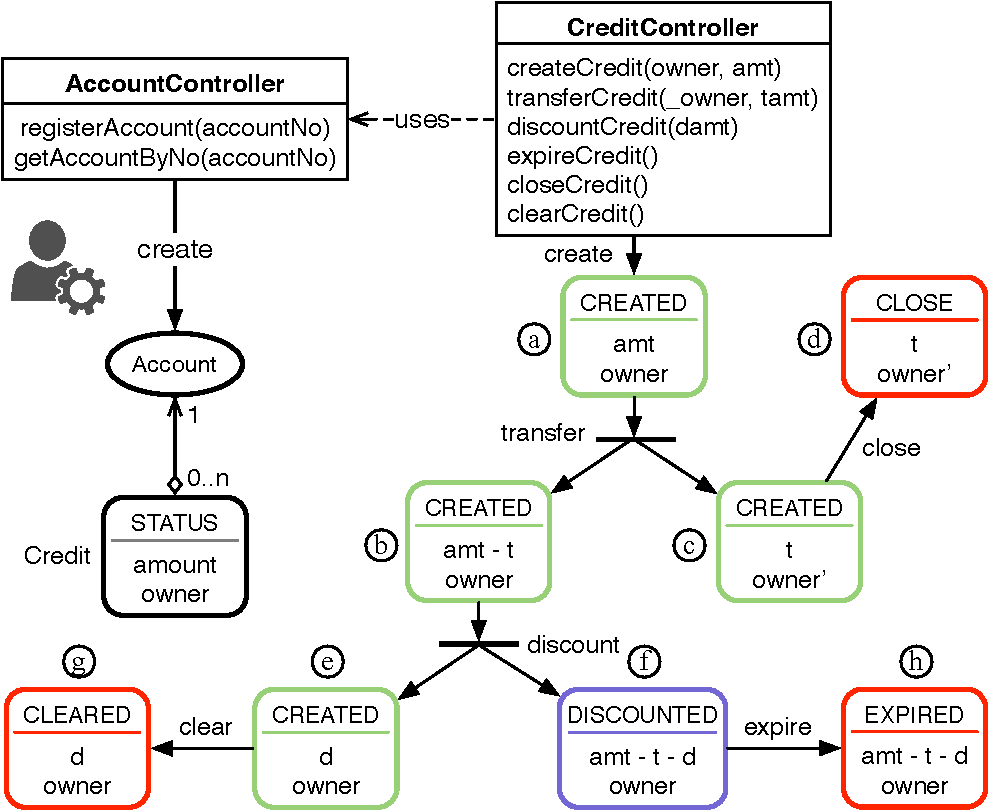
\includegraphics[width=.80\columnwidth]{Figures/Chapter3/modcon.pdf}
	\caption{Illustration of a \wecredit smart contract at \company.}
	\label{fig:scenario}
\end{figure}

The user first deploys an \code{AccountController} contract, whose address is then used to
instantiate the \code{CreditController} contract.
\code{AccountController} is in charge of the account creation and management.
An account may own \code{Credit}(s), which are transferable and divisible tokens with stipulated values.
The state of a \code{Credit} is captured by the tuple, $(\mathit{STATUS},amount,owner)$, whose
fields represent the status, value captured, and its ownership, respectively.
A \code{Credit} instance supports credit operations including creation, transfer, discount, expiration, clearance, and closure.
Through \code{CreditController}, one can first create a credit, namely, \textcircled{a},
under the specified \code{Account}.
In this case, a \code{transfer} operation is executed on \textcircled{a}, thus dividing
\textcircled{a} into two new credits, namely, \textcircled{\raisebox{-.9pt}{b}} and \textcircled{c}.
By design, the total value of \textcircled{\raisebox{-.9pt}{b}} and \textcircled{c} equals to that
of \textcircled{a}.
Then a \code{discount} operation is applied on \textcircled{\raisebox{-.9pt}{b}}, resulting in
a newly created credit \textcircled{e} and a discounted credit \textcircled{\raisebox{-.9pt}{f}}.
By design, the total value of \textcircled{e} and \textcircled{\raisebox{-.9pt}{f}} equals to that
of \textcircled{\raisebox{-.9pt}{b}}, but the status of \textcircled{\raisebox{-.9pt}{f}} becomes
``DISCOUNTED''. %which is different from \textcircled{\raisebox{-.9pt}{e}} marked as ``CREATED''.
To complete the life cycle of a credit, one may apply either the \code{close}, \code{clear}, or
\code{expire} operation, bringing the credit into the ``CLOSED'' (e.g.,
\textcircled{\raisebox{-.9pt}{d}}), ``CLEARED'' (e.g., \textcircled{\raisebox{.9pt}{g}}), or
``EXPIRED'' (e.g., \textcircled{\raisebox{-.9pt}{h}}) state, respectively.
Once a credit is in ``CLOSED\allowbreak{}/CLEARED\allowbreak{}/EXPIRED'', it should no longer
accept further operation.

%\yi{Let's not focus on FISCO BCOS so much. In principle, the modcon also work on Ethereum. We just
%use FISCO as an industrial case study.}
%FISCO BCOS~\cite{fisco} is a secure and reliable financial-grade open-source blockchain platform
%led by Chinese enterprises.
%Its performance, usability, and security have been testified by many institutional users and
%successful business applications in a live production environment.
%FISCO BCOS has been adopted in over 10 applications in areas like government affairs, finances,
%charity, health care, education, transport, copyright, product tracing, supply chain, recruitment,
%agriculture, social communication, and entertainment.
%\par

%Smart contracts are at the core of these applications on FISCO BCOS blockchain.
%Similar to Ethereum, FISCO BCOS supports writing smart contract using Solidity programming
%language.
%Since writing secure smart contract is non-trivial, which requires programmers have a comprehensive
%understanding of smart contract language and blockchain platform principles, etc,
%there are considerable number of smart contract attacks~\textcolor{red}{XXX atacks} in recent
%years.
%Testing or verifying smart contracts appeals greatly to the research
%community~\textcolor{red}{Testing or verifying researches}.

Existing testing and analysis tools target Ethereum smart contracts and mainly focus on their
security issues.
Such tools do not work well on this example for the following reasons.
\textbf{(1) Lack understanding of system behaviors}.
The different states of a credit instance is implemented with special encoding.
For example, the $\mathit{STATUS}$ field is encoded as bit-vectors for performance considerations.
It is unclear how to interpret system states and behaviors at these states without this knowledge.
\textbf{(2) Absence of oracle}.
Existing tools may rely on implicit security properties (e.g., underflow/overflow and exceptions)
as oracle, which is absent when the functional correctness is concerned.
The expected system behavior (e.g., ``EXPIRED'' is terminal) is not known prior and should be
provided by the contract designer.
\textbf{(3) Missing measurement of test adequacy}.
The traditional coverage criteria used by existing tools, such as branch and path coverage, are not
good measurement of test adequacy for this example.
Covering every single path of the contract program does not equal exercising all system states and
state transitions.
It is challenging to navigate through all system behaviors without proper adequacy measurements.

%\yi{Let's not sell FISCO BCOS, which is not so well-known. The selling point should be model-based
%testing.}
%However, most existing research tools support only testing smart contract on Ethereum.
%Smart contracts on FISCO BCOS are industrial applications of high complexity and high value beyond
%those on Ethereum.
%Generating smart contracts automatically could ensure the security of smart contracts to some
%extent by well-defined formal models such as state machine model \textcolor{red}{ref}.
%However, most available smart contracts are usually not generated full-automatically by model
%specification.
%Testing remains an effective measure to verify whether there is any violation against model
%specification of smart contract.
%\par

\paragraph{\modcon}
To address these challenges, we propose \modcon, a model-based testing platform for smart contracts.
\modcon targets enterprise smart contract applications written in Solidity~\cite{solidity} from permissioned/consortium blockchains such as FISCO BCOS, but is also compatible with Ethereum.

\modcon allows users to specify system models and define test oracles, which are then used to guide
the test generation and execution.
%which firstly supports FISCO BCOS (\textcolor{red}{not sure as well as Ethereum}).
%\modcon is a Web-based testing framework, which provides basic workflow( Uploading, Compiling,
%Deployment, Query/Transaction ) to interact with smart contracts on FISCO BCOS.
%\modcon enables smart contract testing once user provides the model specification of smart contract
%while \modcon allows for testing strategy or test case priority specified by user.
The key features of \modcon include test-model specification, customized test generation and user friendly web-based interface.

\subsection{\modcon Overview}
\label{sec:Overview}

\begin{figure}[t]
	\centering
	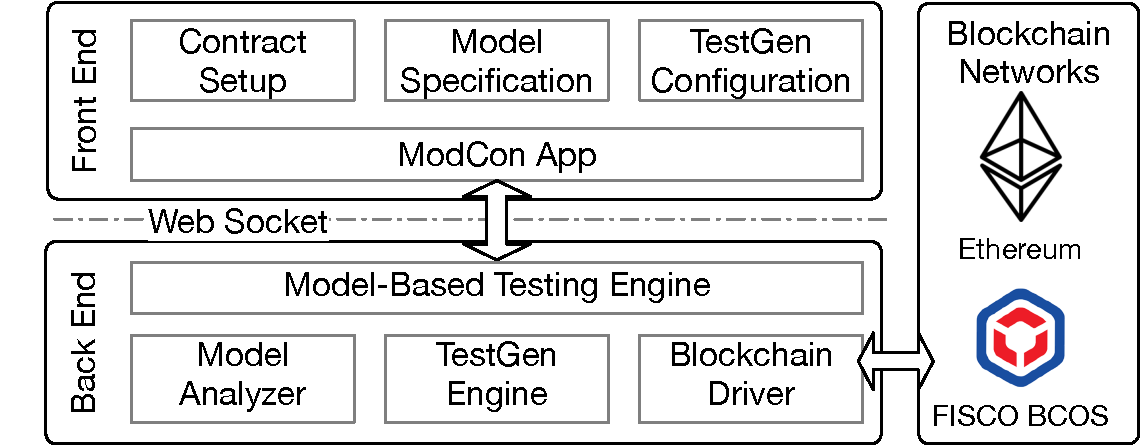
\includegraphics[width=.9\columnwidth]{Figures/Chapter3/modcon-arch.pdf}
	\caption{Architecture of \modcon.}
	\label{fig:architecture}
\end{figure}

In this section, we describe the architecture of \modcon and demonstrate its user interface.
As shown in \cref{fig:architecture}, \modcon consists of a web-based front end (implemented as a
Vue.js~\cite{vuejs} application) and a server-side back end (implemented on top of the Node.js
JavaScript runtime~\cite{nodejs}).
The front-end accepts two inputs from users: the target smart contracts
%which will then be compiled by \modcon and deployed to blockchain platforms.
and the test-model specifications to drive the model-based testing process.
The front-end allows users to specify coverage strategies and configure test generation priority,
and the test execution progress can be monitored on-the-fly.
The back-end communicates with the front-end through the WebSocket.
On the back-end, the model-based testing engine is in charge of smart contract
compilation/deployment, model specification analysis, and the customized model-based testing tasks
as per users' requests.

\subsubsection{User Interface}
The user interface of \modcon mainly supports three tasks, namely, contract setup, model
specification, and testing controls.

\begin{figure}[t]
	\centering
	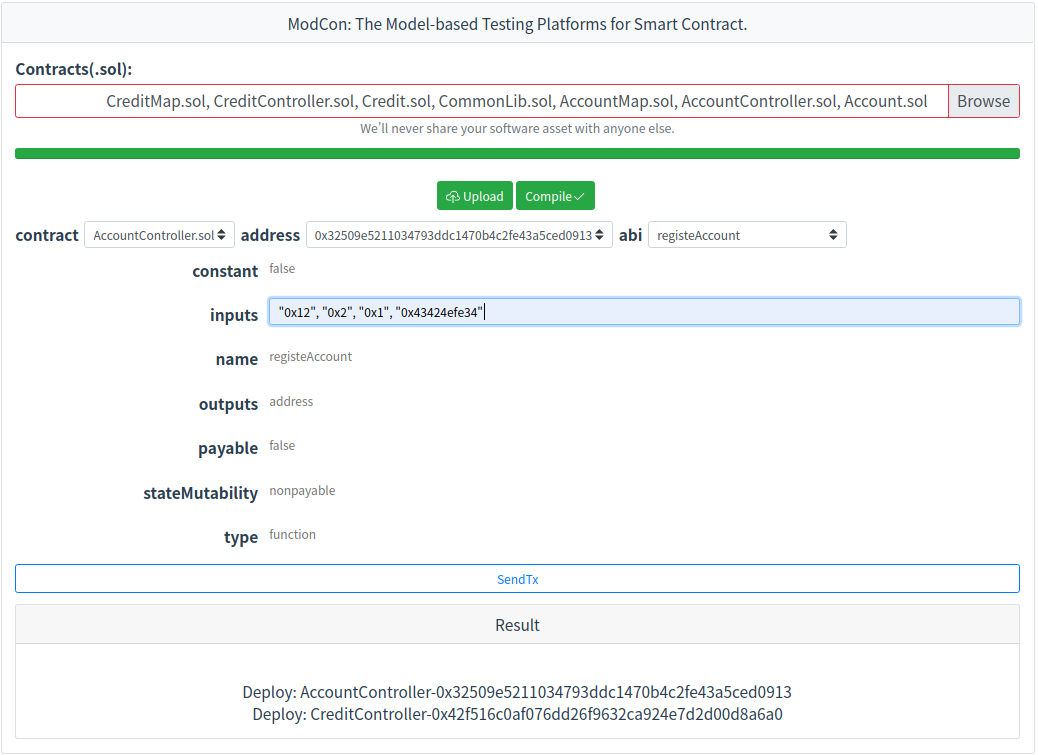
\includegraphics[width=0.90\columnwidth]{Figures/Chapter3/modcon-home.png}
	\caption{Smart contract deployment and setup.}
	\label{fig:modcon-home}
\end{figure}

\paragraph{Contract Setup}
First, users are to upload all relevant smart contract source files, which are then automatically
compiled and deployed onto the blockchain network.
%If there is no compilation error, users can deploy these smart contracts following the on-screen
%guidance.
Once the contracts are successfully deployed, users can directly interact with them by sending
transactions, and the transaction receipts are displayed on the result pane below.
For example, as shown in \cref{fig:modcon-home}, seven contracts related to the \wecredit
application (i.e., \code{Account}, \code{AccountController}, \code{Credit},
\code{CreditController}, ...) had been uploaded to \modcon.
\code{AccountedController} and \code{CreditController} were deployed at addresses,
``\code{0x325...913}'' and ``\code{0x42f...6a0}'', respectively.
One transaction, calling the \code{registerAccount} function, was sent to \code{AccountController}
to create an account which would be used to hold credit instances.
The target contracts' information, including the ABIs and deployment details, are cached and will
be used for test case generation in a later stage.

\begin{figure}[t]
	\centering
	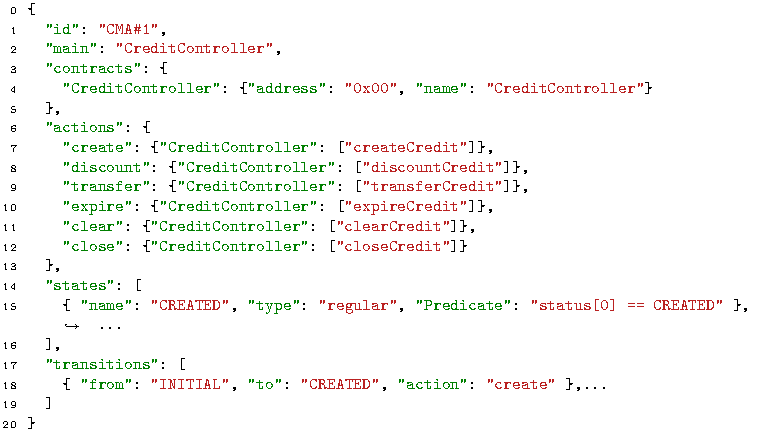
\includegraphics[width=0.9\columnwidth,trim=0 10pt 0 10pt, clip]{Figures/Chapter3/modelSpecification.pdf}
	\caption{User-configured model specification.}
	\label{fig:specification}
\end{figure}

\paragraph{Model Specification}
\Cref{fig:specification} shows an abridged test-model specification for the \wecredit application, which user can customize for his/her applications.
%The specification is explained as follows.
The ``\code{id}'' and ``\code{main}'' fields indicate the model identifier and the entry contract,
respectively.
The ``\code{contracts}'' field lists all relevant contract dependencies required in the test model.
The ``\code{states}'' and ``\code{transitions}'' fields jointly define a state machine model for
the target application.
The ``\code{actions}'' field establish a mapping between functions from the contract implementation
and the actions that can be taken to perform state transitions.

\begin{figure}[t]
	\centering
	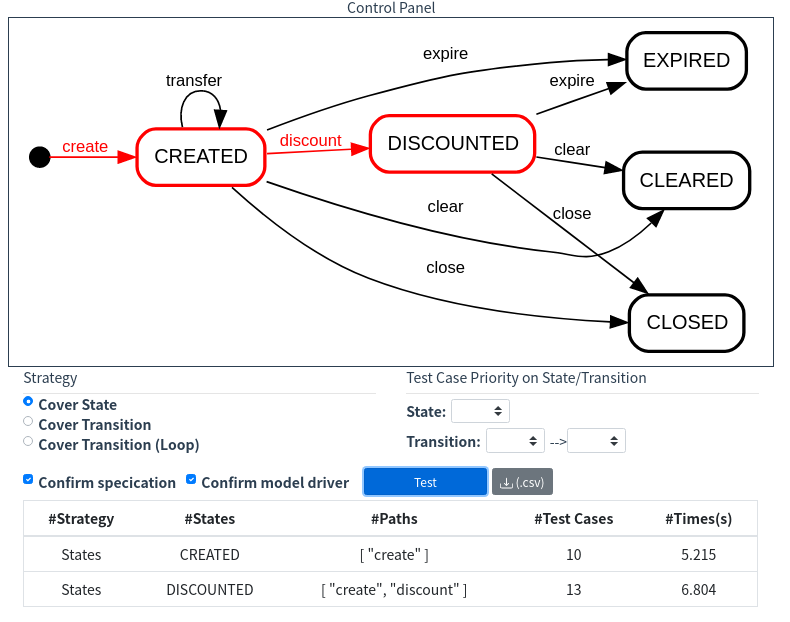
\includegraphics[width=.79\columnwidth]{Figures/Chapter3/modcon-test.png}
	\caption{Test generation control panel.}
	\label{fig:modcon-test}
\end{figure}


\paragraph{TestGen Configuration}
The test-model specification (i.e., \cref{fig:specification}) provided by users is visualized as a
state machine diagram shown in \cref{fig:modcon-test}.
Users may further customize the test generation process by choosing from the three coverage
strategies: (1) \emph{cover states}, aiming to cover every states,
(2) \emph{cover transitions}, aiming to cover every transitions, and
(3) \emph{cover transitions (loop)}, aiming to cover every transitions including loops.
Based on experiments, covering loop transitions may increase testing costs without covering new
states, but it can help discover corner cases and verify the integrity of the test-model.
In addition, users may prioritize the test generation leaning towards specific states or
transitions.
As shows in \cref{fig:modcon-test}, the ``cover states'' strategy is selected and the states
\code{CREATED} and \code{DISCOUNTED} are covered by $10$ and $13$ test cases, respectively.


\subsubsection{Back-End Implementation}
\label{sec:backend}
The model-based testing engine consists of three parts: i.e., model analyzer, test generation
engine, and blockchain driver.

\paragraph{Model Analyzer}
%The model analyzer handles basic contract compilation as well as deployment, as well as
%transactions, and
The model analyzer reads the model specification from the front-end and automatically translates it
into a test driver written in JavaScript.
The test driver stipulates how tests should be generated and executed, which is then displayed in
the front-end client for users' confirmation and customization.
For instance, users may insert additional test oracles in the form of pre/post conditions and
assertions.

%\noindent\textbf{Compiling \& Deployment module.}
\paragraph{TestGen Engine}
The test generation (TestGen) engine receives testing requests and collects the test-model related
information from the front-end, which includes the confirmed test driver, the coverage strategies,
and the test generation priorities.
The engine first computes all logical transition paths following the specific coverage strategies
and goals using graph searching algorithms.
For example, to reach the \code{CLEARED} state of \wecredit shown in \cref{fig:modcon-test}, the
logical transition paths for different strategies are listed below.

{\small\begin{itemize}[leftmargin=*,topsep=2pt]
		\item Cover states: INITIAL $\rightarrow$ CREATED $\rightarrow$ CLEARED.
		\item Cover transitions: INITIAL $\rightarrow$ CREATED $\rightarrow$ CLEARED; INITIAL $\rightarrow$
		CREATED $\rightarrow$ DISCOUNTED $\rightarrow$ CLEARED.
		\item Cover transitions (loop): INITIAL $\rightarrow$ CREATED $\rightarrow$ CREATED $\rightarrow$
		CLEARED;
		INITIAL $\rightarrow$ CREATED $\rightarrow$ CREATED $\rightarrow$ DISCOUNTED $\rightarrow$ CLEARED.
\end{itemize}}

The TestGen engine ranks these logical transition paths based on the order defined by the test
case priorities, and then generates concrete test cases (with concrete input values and environment
settings) corresponding to each logical transition path.
The generation of concrete input values adopts standard
techniques, such as the mutation-based method in ContraMaster~\cite{wang2019vultron,wang2019oracle},
with seed pools for different input types.
Built upon the blockchain driver, the TestGen engine sends these concrete test cases to blockchain
platforms for execution and monitors the execution status at the same time.
The engine keeps generating test cases for execution until the maximum time budget or failure
limit is reached.
During test execution, the engine reports the testing results back to the front-end client, which
displays the current progress in real-time.

%\lsw{Do we need to mention how the concrete test cases are generated? Maybe one or two sentences?}\liu{The engine generates concrete test input values using a random method, where all test cases to generate share same random seeds pool because for model-driven smart contracts, along one logical transition path, test cases to different transition are highly related.}


\paragraph{Blockchain Driver}
The blockchain driver directly interacts with the blockchain networks for contract deployment and
establishes a transaction interface with the networks.
Currently, \modcon supports two blockchain platforms, namely, Ethereum and FISCO BCOS.
It can easily be extended to other blockchain platforms.
%The instances can be indexed from contract name without much effort, and the driver ensures that the indexed are the latest instance of contract.


\subsection{Evaluation}
\label{sec:eval}

In this section, we evaluate \modcon on the \wecredit smart contract application from \company and
the \code{BlindAuction} contract used by FSolidM~\cite{mavridou2018designing}, a state machine
based smart contract code generator.

%The case \code{StateMachine} from official Solidity document are also evaluated.
We manually constructed their model specifications with the help from the contract developers and
the related documentation.
The experiments were conducted on a desktop computer with Ubuntu 18.10 OS, an Intel Core i5 $2.50$~GHz processor and $8$GB RAM.
All cases were evaluated on the FISCO BCOS blockchain.

\begin{figure}[t]
	%	\label{fig:cma}
	\centering
	
	\begin{subfigure}[b]{0.47\columnwidth}
		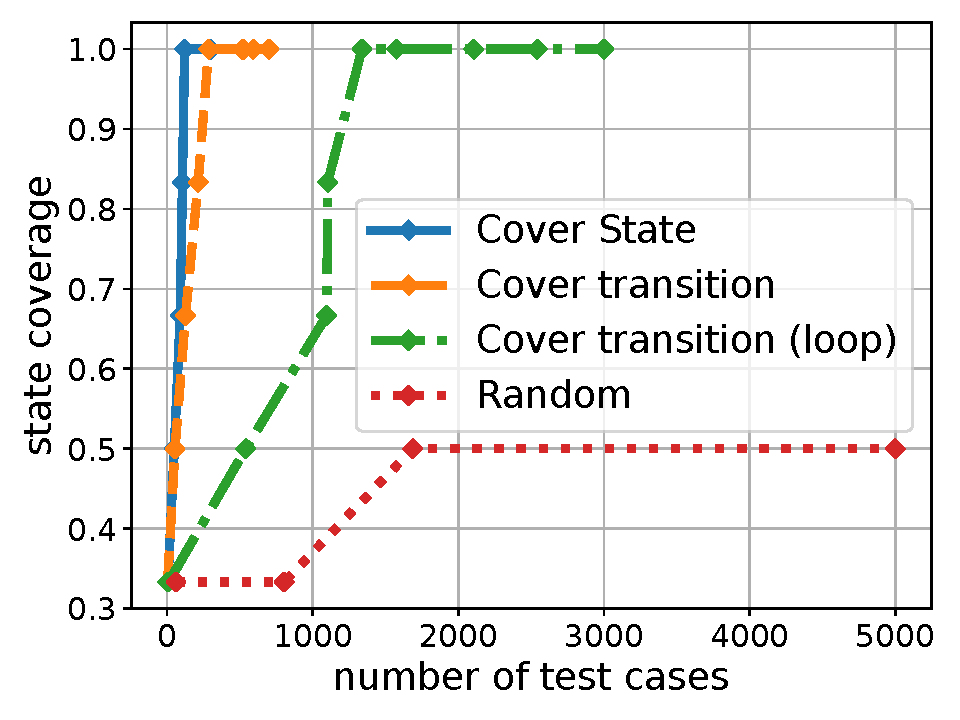
\includegraphics[width=\columnwidth]{Figures/Chapter3/CMA-state-coverage.pdf}
		\caption{\wecredit: state cov.}
		\label{fig:cma-state}
	\end{subfigure}
	\begin{subfigure}[b]{0.47\columnwidth}
		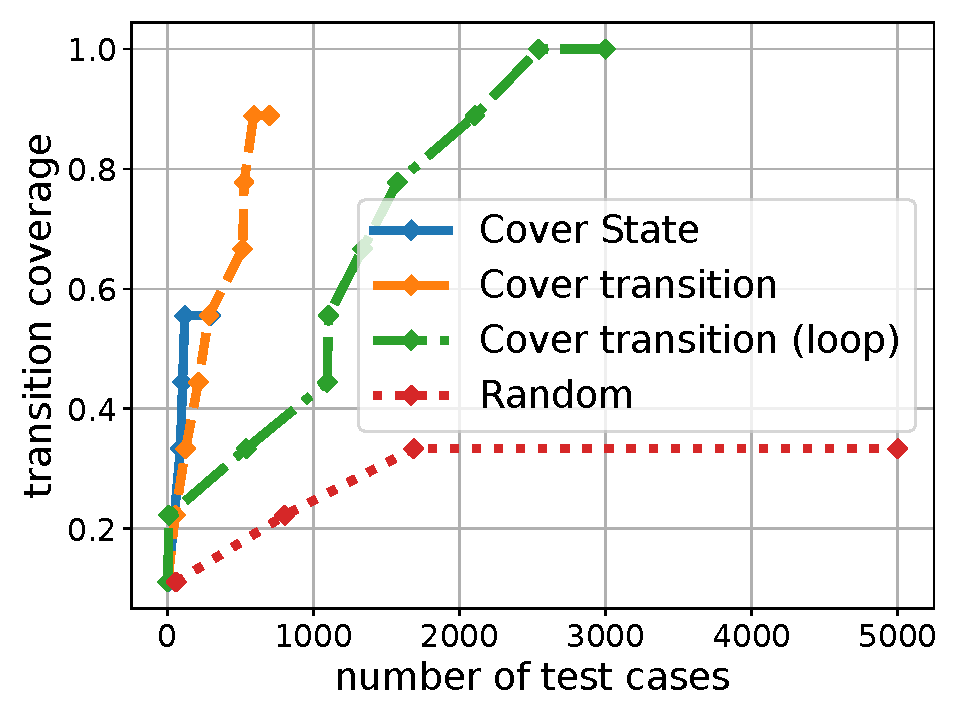
\includegraphics[width=\columnwidth]{Figures/Chapter3/CMA-transition-coverage.pdf}
		\caption{\wecredit: transition cov.}
		\label{fig:cma-transition}
	\end{subfigure}
	\begin{subfigure}[b]{0.47\columnwidth}
		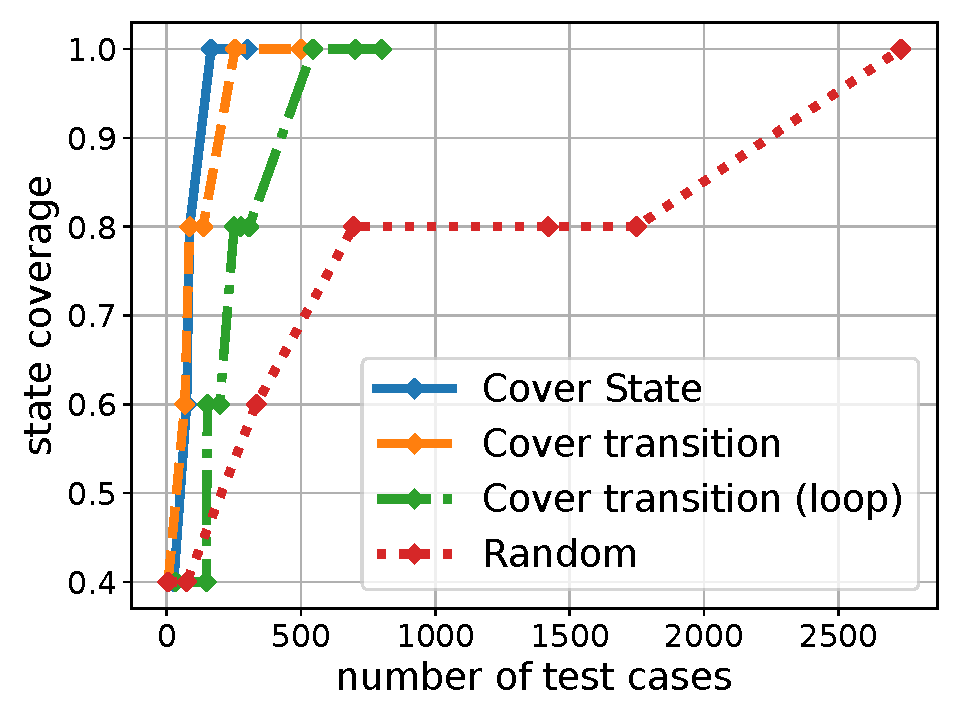
\includegraphics[width=\columnwidth]{Figures/Chapter3/BlindAuction-state-coverage.pdf}
		\caption{\code{BlindAuction}: state cov.}
		\label{fig:auction-state}
	\end{subfigure}
	\begin{subfigure}[b]{0.47\columnwidth}
		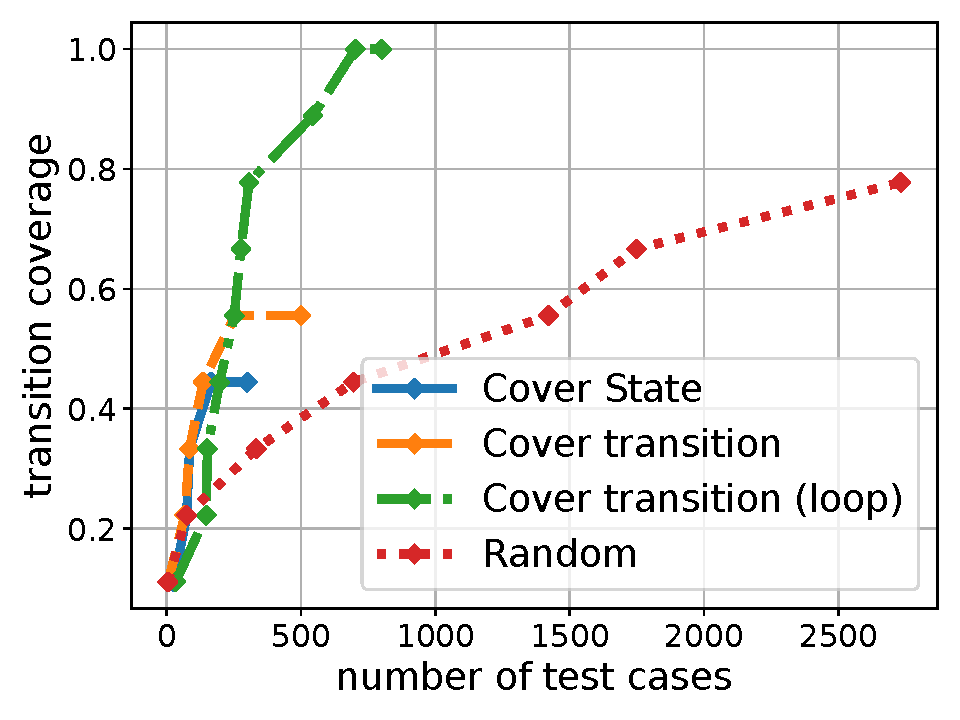
\includegraphics[width=\columnwidth]{Figures/Chapter3/BlindAuction-transition-coverage.pdf}
		\caption{\code{BlindAuction}: transition cov.}
		\label{fig:auction-transition}
	\end{subfigure}
	\caption{State and transition coverage achieved for \wecredit and
		\code{BlindAuction}.}\label{fig:coverage}
%	\caption{State and transition coverage achieved per test for \wecredit and
%		\code{BlindAuction}.}\label{fig:coverage}
\end{figure}

%\begin{figure}[ht]
%%	\label{fig:blindAuction}
%	\centering
%
%	\caption{State and transition coverage of BlindAuction.}
%\end{figure}

\Cref{fig:coverage} shows the evaluation results.
The vertical and horizontal axes represent the state/transition coverage and the number of test
cases, respectively.
We examined aforementioned three coverage strategies and compared the results of \modcon with random
testing.
Among these strategies, the results show that the cover state strategy first reaches all states
of both \wecredit and \code{BlindAuction}, while the strategy to cover transition including loops
has the potential to reach all states and explore more transitions at the cost of more test cases.
All of the three proposed strategies achieve much higher state and transition coverage than random
testing, which shows that random testing is not suitable to deal with enterprise smart contract applications.
Random testing achieves lower state and transition coverage in \wecredit than those in
\code{BlindAuction}, because the former is of higher complexity in its business logic and state encoding than the latter.
%has more states and transitions than the latter.
For example, \wecredit uses a bit-vector of more than 11 bits as its function input or to encode the
$\mathit{STATUS}$, and blindly enumerating bit-vector values is extremely inefficient.

In our experiments, \modcon was able to reach all states and transitions for each case within about
500 test cases.
This is mainly because of the guidance from the test-model, which makes \modcon effective on
enterprise smart contract applications such as \wecredit.
Additionally, with the test-model specification, \modcon allows users to define test oracles in the
generated test driver.
For example, the specification of \wecredit requires \code{CLOSED}, \code{CLEARED}, and
\code{EXPIRED} to be final states, which means no transition shall be made once the system falls
into one of the three states.
We insert this specification as a test oracle into the test driver and discovered violations
against it in the original implementation of \wecredit.
The transitions between \code{EXPIRED}, \code{CLOSED}, and \code{CLEARED} were possible due to an
implementation error.
We reported this error to the \wecredit developer team from \company, and they confirmed it to be a
real bug.
The demonstration video of \modcon, along with more cases and experiment results, can be accessed at: \modconurl.

\subsection{Related Work}
\label{sec:related_work}

%Smart contract development is very different from traditional programming such that developers
%tend
%to write vulnerable smart
%contracts~\cite{delmolino2016step,atzei2016survey,wohrer2018smart,ellul2018runtime}.
Most of the existing testing and analysis tools focus on the security issues of Ethereum smart
contracts.
Oyente~\cite{oyente,luu2016making} is one of the first static analyzer detecting security
vulnerabilities in smart contracts based on symbolic execution.
It searches for violations of predefined security properties without actually executing the
contract program.
Other notable static security analysis tools include Zeus~\cite{kalra2018zeus},
Mythril~\cite{mythril}, sCompile~\cite{chang2018scompile}, and Securify~\cite{tsankov2018securify}.
In contrast, the dynamic tools instrument either the contract code or the Ethereum Virtual Machine
(EVM) and observe anomalies during runtime execution.
ContractFuzzer~\cite{jiang2018contractfuzzer} is the earliest dynamic fuzz testing tool aiming a
number of common vulnerability types, including the reentrancy, exception disorder, block
dependency, etc.
Other fuzzing tools follow similar principles: e.g., Reguard~\cite{liu2018reguard},
ContraMaster~\cite{wang2019vultron,wang2019oracle}, and sFuzz~\cite{nguyen2020sfuzz}.
% arose as the first industrial security analysis tool for Ethereum smart contracts, which combined
% concolic analysis and taint analysis with control flow checking to detect  nearly 30 classes of
% vulnerabilities.
%Also, there are many works resorting to programming analysis technique to detect the
%vulnerabilities of smart contract~\cite{SmartCheck} and empirical
%analysis~\cite{parizi2018empirical} to the tools mentioned above.
These tools are not designed for testing functional correctness, and as mentioned in \cref{sec:intro}, they are not suitable for enterprise smart contract applications
either.

There are several recent works on the functional correctness of Ethereum smart contracts.
VeriSol~\cite{born2020formal} relies on formal verification to check the semantic conformance
between a contract implementation and its workflow policy.
The policy is provided by users, describing the high-level workflow of the application in a style
similar to our model specifications.
FSolidM~\cite{mavridou2018designing} and VeriSolid~\cite{Mavridou2019} both aim to facilitate the
creation of correct-by-design contracts, with emphases on the security and functional aspects,
respectively, 
where a finite state machine is used as the contract specification to capture the expected system behaviors.
\modcon is based on the idea of model-based testing~\cite{utting2012taxonomy}, which uses an explicit
abstract model of the target contract to automatically derive tests.
It serves as a complement to other static validation/construction techniques in providing more
flexible and accurate quality assurance solutions.

\subsection{Conclusion}
\label{sec:conclude}

In this section, we described the architecture of \modcon, its user interface, and prominent features.
We also demonstrated the effectiveness of it on real smart contract applications from \company.
The model-based testing capability of \modcon enables it to generate higher-quality test cases for
enterprise smart contracts from permissioned and consortium blockchains.
%Its Web-based interface allows users to easily access the testing services.
%In the future, we plan to extend \modcon's testing capabilities by supporting more blockchain
%platforms, testing strategies and specification templates.

\section{Semantic Test Oracle of Effective Fuzzing}